\documentclass[11pt,a4paper]{article}

% --- Core Typography & Geometry ---
\usepackage[utf8]{inputenc}
\usepackage[margin=1in]{geometry}
\usepackage{amsmath,amssymb,amsfonts}
\usepackage{graphicx}
\usepackage{booktabs}
\usepackage[table]{xcolor}
\usepackage{tabularx}
\usepackage{multirow}
\usepackage{float}
\usepackage{placeins}
\usepackage{microtype}
\usepackage{hyperref}
\usepackage{tikz}
\usetikzlibrary{shapes.geometric, arrows.meta, positioning, shadows}
\usepackage{fancyhdr}
\usepackage{setspace}
\usepackage{enumitem}

% --- Professional Color Palette ---
\definecolor{primaryblue}{RGB}{30, 58, 138}
\definecolor{accentblue}{RGB}{37, 99, 235}
\definecolor{darkslate}{RGB}{15, 23, 42}
\definecolor{lightgrey}{RGB}{248, 250, 252}
\definecolor{bordergrey}{RGB}{203, 213, 225}
\definecolor{tableheader}{RGB}{241, 245, 249}

% --- Hyperlink Setup ---
\hypersetup{
    colorlinks=true,
    linkcolor=primaryblue,
    citecolor=primaryblue,
    urlcolor=accentblue
}

% --- Header & Footer Configuration ---
\pagestyle{fancy}
\fancyhf{}
\rhead{\small \textcolor{gray}{MovieMind: Capstone Project (Milestone 1)}}
\lhead{\small \textcolor{gray}{Dept. of Computer Science \& Engineering}}
\cfoot{\small \thepage}
\renewcommand{\headrulewidth}{0.4pt}

\setstretch{1.15}
\setlength{\parskip}{5pt}

\begin{document}

% ==============================================================================
% TITLE & ACADEMIC COVER BLOCK
% ==============================================================================
\begin{center}
    {\large \textbf{\textcolor{accentblue}{B.TECH MAJOR PROJECT --- MILESTONE 1 EVALUATION (MARKS: 30)}}}\\[0.35cm]
    {\LARGE \textbf{\textcolor{primaryblue}{MovieMind: An Explainable and Conversational Movie Discovery Platform}}}\\[0.25cm]
    {\normalsize \textbf{Department of Computer Science and Engineering}}\\[0.2cm]
    \rule{\linewidth}{1.2pt}\\[0.3cm]
    
    \begin{tabularx}{\textwidth}{lX lX}
        \textbf{Author 1:} & Rajat Verma (\texttt{E23CSEU1490}) & \textbf{Course:} & B.Tech Capstone Project \\
        \textbf{Author 2:} & Alok Verma (\texttt{E23CSEU1489}) & \textbf{Submission:} & October 18, 2026 \\
        \textbf{Author 3:} & Yash Bharadwaj (\texttt{E23CSEU1499}) & \textbf{Live App:} & \url{https://moviemind-eight.vercel.app} \\
        \textbf{Department:} & Computer Science \& Engineering & \textbf{Repository:} & \url{https://github.com/rajatverma777/MovieMind} \\
    \end{tabularx}
    \rule{\linewidth}{0.6pt}
\end{center}

\vspace{0.15cm}

% --- Abstract ---
\begin{abstract}
Digital streaming media fragmentation across platforms (Netflix, Prime Video, Disney+, Apple TV+) has created severe decision fatigue, causing viewers to spend 15 to 20 minutes per session browsing catalogs. Existing commercial systems operate as unexplainable black-box collaborative filters restricted strictly to internal catalogs, while generic Large Language Models (LLMs) suffer from hallucinations and lack verified data grounding. This report presents \textbf{MovieMind}, an explainable, cross-platform movie discovery engine coupled with an agentic conversational AI layer. The system maps verified movie metadata from The Movie Database (TMDB) into a 19-dimensional genre vector space, computing mathematically verifiable Cosine Similarity scores against dynamic candidate pools. Concurrently, Google Gemini Flash (orchestrated via LangChain tool-calling) parses user intent, executes deterministic lookups, and presents structured interactive cards with verified trailers directly in-app. This proposal covers all twelve prescribed Milestone-1 deliverables: problem formulation, UN SDG alignment, literature review, gap analysis, stakeholder and requirements specifications, 4-way feasibility, risk mitigation, full 5-stage methodology, system interaction flowcharts, and a two-milestone execution plan.
\end{abstract}

\vspace{0.25cm}

% ==============================================================================
% 1. FINAL PROBLEM STATEMENT AND MOTIVATION
% ==============================================================================
\section{Final Problem Statement and Motivation}

\subsection{Final Problem Statement}
In the contemporary digital streaming landscape, the rapid proliferation of subscription streaming services has created severe decision fatigue for consumers. Viewers spend between 15 to 20 minutes per viewing session simply browsing through catalogs before either selecting a title or abandoning the session altogether. 

This core challenge is compounded by four specific architectural limitations:
\begin{enumerate}[leftmargin=*]
    \item \textbf{Catalog Siloing:} Streaming recommendation engines are strictly confined to their internal licensed inventory; they never recommend relevant content available on competing services.
    \item \textbf{Algorithmic Opacity (The Black-Box Problem):} Commercial systems rely on proprietary collaborative filtering or deep matrix factorization. Users are offered suggestions without justifiable reasoning, preventing them from understanding or refining their algorithmic profile.
    \item \textbf{Rigid Search Interfaces and LLM Hallucinations:} Traditional discovery relies on static keyword searches or dropdown filters that fail to capture nuanced conversational intent (e.g., \textit{``a slow-burn psychological thriller with a rainy atmosphere''}). Conversely, when users query general-purpose LLMs (such as standalone ChatGPT), the models regularly hallucinate non-existent movie titles, invent release years, and cannot provide verified metadata or streaming availability.
    \item \textbf{Fragmented Trailer Discovery and Video Switching:} Movie trailers and teasers are scattered across external video sites and distributor channels. When discovering a movie, viewers are forced to leave the catalog application, open YouTube, manually search for the official trailer, filter out spoilers or fan-made clickbait cuts, and switch back and forth between multiple applications.
\end{enumerate}

\subsection{Motivation and Objectives}
The motivation behind \textbf{MovieMind} is to build a unified, platform-agnostic, and explainable movie recommendation engine coupled with a conversational AI agent and an all-in-one media preview hub. By mathematically grounding recommendations in a transparent vector space model (Cosine Similarity on 19-dimensional genre distributions), embedding official trailers directly into the discovery flow, and using an LLM strictly as an orchestrator and natural language interface, MovieMind eliminates black-box opacity, stops LLM hallucinations, and provides a frictionless, comprehensive movie exploration experience in a single platform.

% ==============================================================================
% 2. SDG MAPPING AND RATIONALE
% ==============================================================================
\section{UN Sustainable Development Goals (SDG) Mapping and Rationale}

The United Nations Sustainable Development Goals (UN SDGs) provide a benchmark for ethical, sustainable, and socially responsible engineering solutions. MovieMind aligns directly with three targets:

\begin{table}[H]
\centering
\small
\begin{tabularx}{\textwidth}{p{4.2cm} p{3.6cm} X}
\toprule
\rowcolor{tableheader}
\textbf{Target SDG} & \textbf{Specific Target} & \textbf{MovieMind Architectural Rationale} \\
\midrule
\textbf{SDG 9: Industry, Innovation, and Infrastructure} & Target 9.5: Enhance scientific research \& technological innovation & Demonstrates a decoupled hybrid AI paradigm combining mathematical vector algebra with modern generative models deployed on efficient, low-cost serverless microservices. \\
\addlinespace
\textbf{SDG 12: Responsible Consumption and Production} & Target 12.8: Relevant information for sustainable lifestyles & Minimizes computational waste and network bandwidth caused by prolonged, fruitless 20-minute user searches. Employs privacy-preserving client-side storage without centralized data harvesting. \\
\addlinespace
\textbf{SDG 4: Quality Education and Digital Literacy} & Target 4.4: Increase digital literacy and transparent technology & Demystifies recommendation black boxes by displaying explicit Cosine Similarity match percentages (e.g., 82\%) and genre convergence reasons to the user. \\
\bottomrule
\end{tabularx}
\caption{United Nations Sustainable Development Goals (SDG) Alignment Matrix.}
\label{tab:sdg}
\end{table}

% ==============================================================================
% 3. BACKGROUND AND CONTEXT
% ==============================================================================
\section{Background and Context}

Recommender Systems (RS) originated in the early 1990s as an information retrieval mechanism to mitigate digital information overload. The field has evolved through three distinct technical paradigms:
\begin{itemize}[leftmargin=*]
    \item \textbf{Collaborative Filtering (CF):} Predicts preferences based on user-item interaction matrices. While powerful on massive commercial datasets, it suffers from the critical \textit{cold-start problem} (inability to recommend to new users or unrated items) and complete algorithmic opacity \cite{koren2009matrix}.
    \item \textbf{Content-Based Filtering (CBF):} Models items and user profiles as explicit feature vectors in an $N$-dimensional metric space, measuring similarity independently of external user behavior \cite{adomavicius2005toward}.
    \item \textbf{Conversational Recommender Systems (CRS):} Modern architectures that combine conversational natural language interfaces with backend domain databases, allowing dynamic preference elicitation through multi-turn dialogue \cite{fan2023recommender}.
\end{itemize}

MovieMind builds directly upon Content-Based Filtering and CRS by taking verified metadata from \textbf{The Movie Database (TMDB)}, calculating deterministic vector similarities, and wrapping the pipeline in an intelligent conversational agent using \textbf{LangChain} and \textbf{Google Gemini}.

\clearpage
% ==============================================================================
% 4. LITERATURE AND EXISTING-SOLUTION REVIEW
% ==============================================================================
\section{Literature and Existing-Solution Review}

To establish technical grounding, we review foundational literature alongside recent 2023--2025 research on LLM-based recommenders and industrial platforms:

\begin{table}[H]
\centering
\footnotesize
\begin{tabularx}{\textwidth}{p{3.4cm} p{3.2cm} X p{3.6cm}}
\toprule
\rowcolor{tableheader}
\textbf{Study / Platform} & \textbf{Core Methodology} & \textbf{Key Strengths} & \textbf{Identified Limitations Addressed} \\
\midrule
\textbf{Salton \& McGill (1983)} \cite{salton1983introduction} & Vector Space Model (VSM) \& Cosine Similarity & Mathematically proven, bounded ($[0,1]$), low computational complexity $O(n)$. & Operates on static feature arrays; lacks natural language dialogue capabilities. \\
\addlinespace
\textbf{Adomavicius \& Tuzhilin (2005)} \cite{adomavicius2005toward} & Content-Based \& Hybrid Filtering & Solves collaborative cold-start problems; high item independence. & Requires structured taxonomies; lacks conversational preference elicitation. \\
\addlinespace
\textbf{Fan et al. (2023)} \cite{fan2023recommender} & Hybrid LLM + Recommender Integration & Proves that LLMs excel as conversational orchestrators when paired with deterministic tools. & Pure LLM prompting without external tools suffers from high token latency and unverified suggestions. \\
\addlinespace
\textbf{Hou et al. (2024)} \cite{hou2024large} & LLM Zero-Shot Recommendation Benchmark & Evaluates LLM prompting across movie datasets; highlights semantic intent understanding. & Discloses critical \textbf{popularity bias and hallucinations} unless grounded by verified API catalogs. \\
\addlinespace
\textbf{Zhang \& Chen (2023)} \cite{zhang2023explainable} & Explainable AI (XAI) in Recommenders & Demonstrates that feature-level transparency (e.g., genre overlap \%) significantly boosts user trust. & Black-box neural embeddings hide the rationale behind suggestions, degrading user trust. \\
\addlinespace
\textbf{Gomez-Uribe \& Hunt (2015)} \cite{gomez2015netflix} & Deep Matrix Factorization & Highly personalized to watch time; drives 80\%+ of platform streams. & Walled garden (only Netflix titles); complete black-box; lacks cross-platform discovery. \\
\bottomrule
\end{tabularx}
\caption{Comprehensive Review of Relevant Literature and Existing Solutions.}
\label{tab:literature}
\end{table}

\clearpage
% ==============================================================================
% 5. GAP ANALYSIS
% ==============================================================================
\section{Gap Analysis}

A critical review reveals a clear operational void between conventional deterministic database systems and generative AI chatbots:

\begin{table}[H]
\centering
\small
\begin{tabularx}{\textwidth}{p{3.2cm} X X X}
\toprule
\rowcolor{tableheader}
\textbf{Evaluation Dimension} & \textbf{Streaming Services (Netflix/Prime)} & \textbf{Catalog Sites (IMDb/Letterboxd)} & \textbf{Standalone LLMs (ChatGPT/Claude)} \\
\midrule
\textbf{Catalog Scope} & Siloed (in-house titles only) & Global movie database & General static pretraining \\
\textbf{Conversational Flow} & None (grid browsing only) & None (manual filters only) & High natural fluency \\
\textbf{Explainability} & Opaque black-box & User review consensus & Unverified text rationale \\
\textbf{Factual Accuracy} & 100\% internal inventory & 100\% verified database & Low (hallucinates titles/dates) \\
\textbf{In-App Trailers} & Trailer auto-play (internal) & External clip links & None \\
\midrule
\rowcolor{lightgrey}
\textbf{MovieMind Solution} & \multicolumn{3}{l}{\textbf{Unified Catalog (850k+ films) + Verifiable Cosine Math + Zero-Hallucination Chat + Unified Trailers}} \\
\bottomrule
\end{tabularx}
\caption{Gap Analysis Matrix Comparing MovieMind Against Current Market Solutions.}
\label{tab:gap}
\end{table}

\textbf{Core Gaps Addressed by MovieMind:}
\begin{enumerate}[leftmargin=*]
    \item \textbf{The Transparency Gap:} Commercial platforms treat user recommendations as a fait accompli. MovieMind exposes the exact mathematical overlap score and genre rationale.
    \item \textbf{The Verification Gap:} Vanilla LLMs guess titles; MovieMind forces the model to call deterministic lookup tools, guaranteeing 100\% of suggested films exist on TMDB.
    \item \textbf{The Preview Fragmentation Gap:} MovieMind integrates official YouTube trailer playback directly into the film modal, eliminating disruptive app-switching.
\end{enumerate}

% ==============================================================================
% 6. CUSTOMER / USER REQUIREMENTS, FUNCTIONAL AND NON-FUNCTIONAL REQUIREMENTS
% ==============================================================================
\section{Customer / User Requirements, Functional and Non-Functional Requirements}

\subsection{Customer and Target User Personas}
\begin{itemize}[leftmargin=*]
    \item \textbf{Persona A --- Casual Weekend Viewer:} Seeks immediate, high-confidence recommendations with embedded trailers to make decisions in $< 2$ minutes without navigating multiple streaming accounts.
    \item \textbf{Persona B --- Cinephile / Power User:} Demands specific thematic queries (e.g., \textit{``atmospheric cyberpunk neo-noir like Blade Runner''}), transparent match percentages, and local watchlist curation.
    \item \textbf{Persona C --- Privacy-Conscious User:} Refuses to register accounts or endure behavioral tracking; requires all personal viewing data to reside strictly on their own browser.
\end{itemize}

\subsection{Functional Requirements (FR)}
\begin{itemize}[leftmargin=*]
    \item \textbf{FR-01 (Dynamic Catalog Ingestion):} The system shall fetch and render live Trending, Top-Rated, and Now-Playing films from TMDB REST endpoints.
    \item \textbf{FR-02 (Instant Keyword Search):} The system shall provide sub-second search capabilities by movie title and thematic keyword.
    \item \textbf{FR-03 (Unified Trailer Playback):} The system shall embed and play official HD YouTube trailers directly inside the movie details modal.
    \item \textbf{FR-04 (Client Watchlist Persistence):} The system shall enable users to bookmark films into a local watchlist stored privately via browser Web Storage (LocalStorage).
    \item \textbf{FR-05 (19-Dimensional Vector Mapping):} The system shall transform categorical genre arrays into 19-dimensional binary vectors matching TMDB taxonomy.
    \item \textbf{FR-06 (Cosine Similarity Scoring):} The recommendation module shall compute normalized dot product similarity scores against candidate pools.
    \item \textbf{FR-07 (Conversational Dialogue):} The system shall process multi-turn natural language queries and return structured JSON cards with match percentages and explanations.
\end{itemize}

\subsection{Non-Functional Requirements (NFR)}
\begin{itemize}[leftmargin=*]
    \item \textbf{NFR-01 (Performance and Latency):} Vector similarity math must execute in $< 100\text{ ms}$; total conversational AI response time must not exceed $3.0\text{ seconds}$.
    \item \textbf{NFR-02 (Security and Key Isolation):} API secrets (\texttt{GEMINI\_API\_KEY}, \texttt{TMDB\_API\_KEY}) must reside exclusively on serverless runtimes and never leak into client JavaScript bundles.
    \item \textbf{NFR-03 (Fault Tolerance):} Automatic multi-tier failover must handle API rate limits (HTTP 429) or cloud outages without crashing the client.
    \item \textbf{NFR-04 (Privacy by Design):} The application shall not store personally identifiable information (PII) on centralized servers without explicit consent.
    \item \textbf{NFR-05 (Responsive Usability):} The interface must be fully responsive across mobile, tablet, and desktop viewports following dark-theme UI standards.
\end{itemize}

\clearpage
% ==============================================================================
% 7. TECHNOLOGY AND TOOL SELECTION WITH JUSTIFICATION
% ==============================================================================
\section{Technology and Tool Selection with Justification}

\begin{table}[H]
\centering
\small
\begin{tabularx}{\textwidth}{p{3.0cm} p{3.2cm} X p{3.5cm}}
\toprule
\rowcolor{tableheader}
\textbf{Layer} & \textbf{Selected Tool} & \textbf{Technical Justification} & \textbf{Rejected Alternatives} \\
\midrule
\textbf{Frontend} & React 18 + Vite & Fast virtual DOM reconciliation, component reactivity, ultra-light bundle ($< 100\text{ kB}$). & Angular (overly heavy); Next.js (unnecessary SSR overhead for discovery client). \\
\addlinespace
\textbf{Backend Proxy} & Node.js Serverless & Non-blocking event loop, sub-second spin-up on Vercel Edge, zero idle server cost. & Django/Flask (slower cold-starts on serverless runtimes). \\
\addlinespace
\textbf{Knowledge Base} & TMDB REST API & 850,000+ film records, verified CDN posters, standardized 19-genre taxonomies, video keys. & OMDB (lacks deep genre arrays); IMDb scraping (violates terms of service). \\
\addlinespace
\textbf{AI Model} & Google Gemini 3.5 Flash & Low-latency inference, native JSON schema mode, multi-turn context, low token cost. & OpenAI GPT-4 (significantly higher cost/latency); Claude (region restrictions). \\
\addlinespace
\textbf{AI Orchestration} & LangChain (\texttt{@langchain/core}) & Standardized message schemas, tool binding, Zod output validation. & Raw SDK prompting (brittle JSON parsing, difficult history management). \\
\addlinespace
\textbf{Client State} & Browser LocalStorage & Instant $O(1)$ read/write latency, zero database maintenance costs, zero user tracking. & MongoDB/Firebase (adds unnecessary auth friction for Milestone 1). \\
\bottomrule
\end{tabularx}
\caption{Technology Selection Matrix with Architectural Justification.}
\label{tab:tech}
\end{table}

% ==============================================================================
% 8. TECHNICAL, ECONOMIC, OPERATIONAL, AND LEGAL/ETHICAL FEASIBILITY
% ==============================================================================
\section{Technical, Economic, Operational, and Legal/Ethical Feasibility}

\begin{itemize}[leftmargin=*]
    \item \textbf{Technical Feasibility (High):} Vector algebra (Cosine Similarity) executes in $O(n)$ time complexity (microseconds in V8 JavaScript). The LangChain and Google GenAI SDKs provide robust tool-calling support with Zod schema validation.
    \item \textbf{Economic Feasibility (High):} The architecture operates completely within free-tier operational limits: Vercel Hobby hosting (\$0), TMDB Developer API (\$0), Google Gemini API free-tier allowances (\$0), and client-side storage (\$0).
    \item \textbf{Operational Feasibility (High):} As a responsive single-page application (SPA), MovieMind requires zero native client downloads and runs seamlessly on all modern web browsers across desktop and mobile devices.
    \item \textbf{Legal and Ethical Feasibility (High):} The application strictly consumes metadata and promotional video IDs licensed under TMDB terms with proper attribution. It does not pirate or host media files, and client-side storage protects user privacy.
\end{itemize}

% ==============================================================================
% 9. SCOPE AND LIMITATIONS
% ==============================================================================
\section{Scope and Limitations}

\subsection{In-Scope Capabilities}
\begin{itemize}[leftmargin=*]
    \item Real-time metadata ingestion from TMDB for global movie titles.
    \item 19-dimensional binary genre vector space modeling with user taste centroid calculation.
    \item Bounded Cosine Similarity scoring ($S \in [0.0, 1.0]$) and ranking.
    \item Conversational chat interface powered by LangChain and Gemini Flash.
    \item In-app YouTube trailer streaming via embedded modal players.
    \item LocalStorage-based watchlist bookmarking and taste persistence.
\end{itemize}

\subsection{Limitations and Out-of-Scope Items}
\begin{itemize}[leftmargin=*]
    \item \textbf{No Video Hosting/Streaming:} MovieMind is strictly a recommendation and discovery portal; it does not host, pirate, or stream full-length films.
    \item \textbf{Third-Party API Dependency:} System uptime is inherently tied to the external availability of TMDB and Google AI Studio APIs.
    \item \textbf{Language Scope:} The primary recommendation and conversational models are tuned for English metadata in this development phase.
\end{itemize}

% ==============================================================================
% 10. RISK ANALYSIS AND MITIGATION STRATEGY
% ==============================================================================
\section{Risk Analysis and Mitigation Strategy}

\begin{table}[H]
\centering
\small
\begin{tabularx}{\textwidth}{p{3.5cm} p{1.6cm} p{1.8cm} X}
\toprule
\rowcolor{tableheader}
\textbf{Risk Category} & \textbf{Severity} & \textbf{Likelihood} & \textbf{Engineered Mitigation Strategy} \\
\midrule
\textbf{Gemini Quota Exceeded (HTTP 429)} & High & Medium & \textbf{Dual-Model Failover:} Primary queries execute on \texttt{gemini-3.5-flash}; on error, the system automatically retries with \texttt{gemini-2.5-flash-lite}. If cloud AI fails, it gracefully falls back to the deterministic local engine. \\
\addlinespace
\textbf{TMDB API Latency} & Medium & Medium & \textbf{In-Memory Caching:} 15-minute in-memory candidate pool cache on the serverless backend to eliminate redundant network roundtrips. \\
\addlinespace
\textbf{LLM Hallucinations} & High & Low & \textbf{Tool-Calling Architecture:} The model is strictly prohibited from generating movie titles directly; it must invoke the verified \texttt{recommend\_movies} tool. \\
\addlinespace
\textbf{API Key Exposure} & Critical & Low & \textbf{Serverless Isolation:} All private keys reside exclusively in server-side environment variables (\texttt{process.env.GEMINI\_API\_KEY}). \\
\bottomrule
\end{tabularx}
\caption{Project Risk Analysis and Engineered Mitigation Matrix.}
\label{tab:risk}
\end{table}

\clearpage
% ==============================================================================
% 11. PROPOSED SOLUTION AND DETAILED METHODOLOGY
% ==============================================================================
\section{Proposed Solution and Detailed Methodology}

\subsection{Five-Stage Engineering Methodology}
MovieMind employs a modular 5-stage pipeline separating data ingestion, mathematical feature engineering, conversational intelligence, and media presentation:
\begin{enumerate}[leftmargin=*]
    \item \textbf{Stage 1 (Data Ingestion \& Live Normalization):} Real-time querying of TMDB endpoints (\texttt{/trending}, \texttt{/now\_playing}, \texttt{/search}, \texttt{/videos}). Payloads are normalized into uniform records with official YouTube trailer keys.
    \item \textbf{Stage 2 (Feature Engineering \& 19-Dim Vector Space):} Categorical genre IDs are mapped into a binary feature vector $\vec{V}_M \in \{0, 1\}^{19}$ based on TMDB's standard taxonomy:
    \[
    \text{GID} = [28, 12, 16, 35, 80, 99, 18, 10751, 14, 36, 27, 10402, 9648, 10749, 878, 10770, 53, 10752, 37]
    \]
    \item \textbf{Stage 3 (Taste Profiling \& Cosine Similarity):} For a user watchlist $W = \{M_1, M_2, \dots, M_k\}$, the user taste centroid $\vec{U}$ is computed as:
    \[
    \vec{U} = \frac{1}{|W|} \sum_{M \in W} \vec{V}_M
    \]
    The similarity score $S \in [0.0, 1.0]$ against a candidate film $C$ is computed via Cosine Similarity:
    \begin{equation}
        \text{Cosine Similarity}(\vec{U}, \vec{V}_C) = \frac{\vec{U} \cdot \vec{V}_C}{\|\vec{U}\| \|\vec{V}_C\|} = \frac{\sum_{i=1}^{19} U_i V_{C,i}}{\sqrt{\sum_{i=1}^{19} U_i^2} \cdot \sqrt{\sum_{i=1}^{19} V_{C,i}^2}}
    \end{equation}
    Candidates are ranked in descending order, strictly filtering out previously consumed titles.
    \item \textbf{Stage 4 (Conversational Orchestration via LangChain):} Natural language prompts are parsed by Google Gemini Flash via LangChain. The model dynamically invokes the \texttt{recommend\_movies} or \texttt{search\_movies} tool and returns a structured JSON schema containing match percentages and genre reasoning.
    \item \textbf{Stage 5 (Media Previews \& Privacy Sovereignty):} Renders responsive UI cards with verified posters, match scores, and embedded YouTube trailer playback. Watchlists are stored privately on the client side via browser LocalStorage.
\end{enumerate}

\subsection{Flowchart 1: Website User Interaction Flow}
The complete user browsing, search, trailer preview, and watchlist personalization flow is illustrated below:

\begin{center}
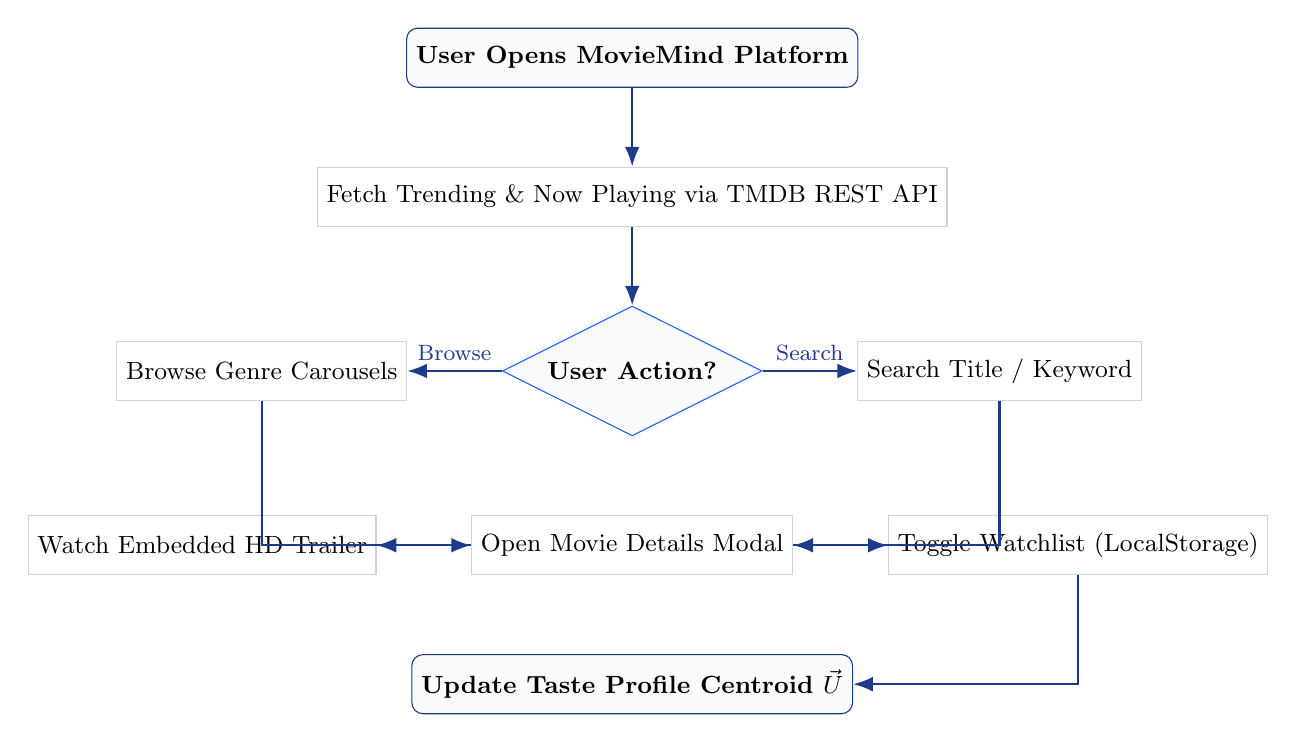
\begin{tikzpicture}[
    node distance=1.0cm and 1.2cm,
    startstop/.style={rectangle, rounded corners, minimum width=3.2cm, minimum height=0.75cm, text centered, draw=primaryblue, fill=lightgrey, font=\small\bfseries},
    process/.style={rectangle, minimum width=3.4cm, minimum height=0.75cm, text centered, draw=bordergrey, fill=white, font=\small},
    decision/.style={diamond, aspect=2, minimum width=2.6cm, text centered, draw=accentblue, fill=lightgrey, font=\small\bfseries},
    arrow/.style={thick, -{Latex[length=2.5mm]}, primaryblue}
]
    \node (start) [startstop] {User Opens MovieMind Platform};
    \node (load) [process, below=of start] {Fetch Trending \& Now Playing via TMDB REST API};
    \node (action) [decision, below=of load] {User Action?};
    \node (browse) [process, left=of action] {Browse Genre Carousels};
    \node (search) [process, right=of action] {Search Title / Keyword};
    \node (modal) [process, below=of action] {Open Movie Details Modal};
    \node (preview) [process, left=of modal] {Watch Embedded HD Trailer};
    \node (watch) [process, right=of modal] {Toggle Watchlist (LocalStorage)};
    \node (update) [startstop, below=of modal] {Update Taste Profile Centroid $\vec{U}$};

    \draw [arrow] (start) -- (load);
    \draw [arrow] (load) -- (action);
    \draw [arrow] (action) -- node[above, font=\footnotesize] {Browse} (browse);
    \draw [arrow] (action) -- node[above, font=\footnotesize] {Search} (search);
    \draw [arrow] (browse) |- (modal);
    \draw [arrow] (search) |- (modal);
    \draw [arrow] (modal) -- (preview);
    \draw [arrow] (modal) -- (watch);
    \draw [arrow] (watch) |- (update);
\end{tikzpicture}
\end{center}

\subsection{Flowchart 2: Conversational AI \& Tool-Calling Pipeline}
The decoupled orchestration between user prompts, the Gemini LLM, LangChain tools, and the deterministic vector engine is outlined below:

\begin{center}
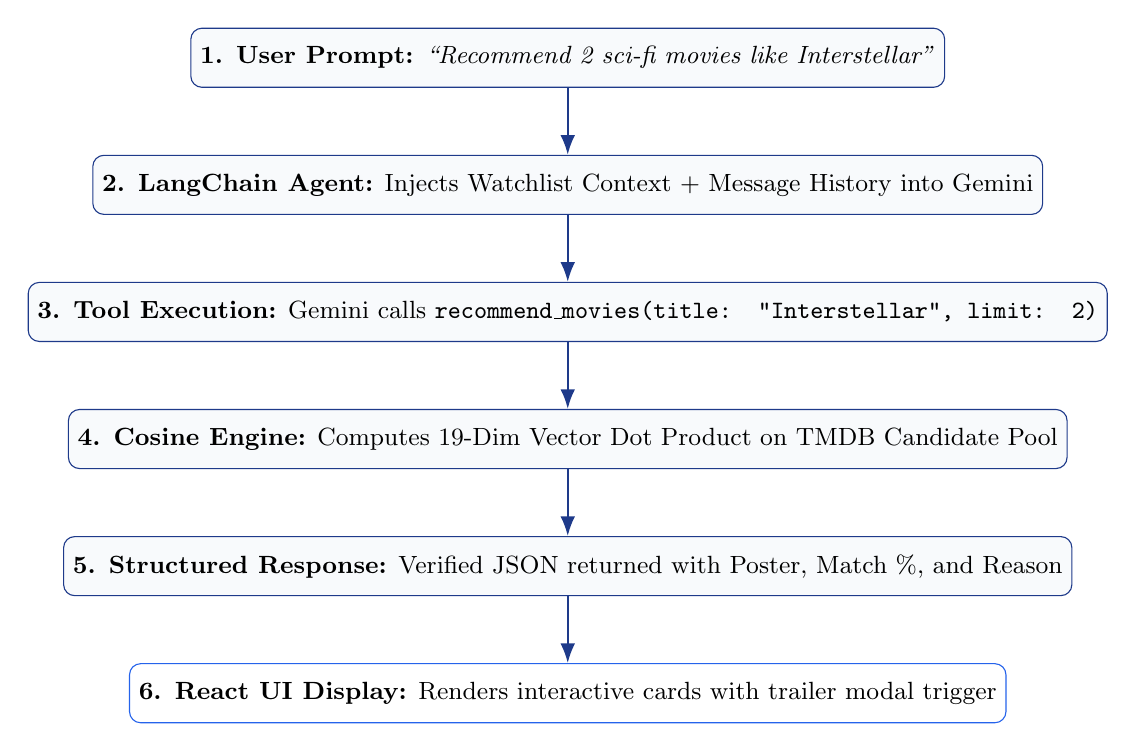
\begin{tikzpicture}[
    node distance=0.85cm,
    stepbox/.style={rectangle, rounded corners=4pt, minimum width=8.5cm, minimum height=0.75cm, text centered, draw=primaryblue, fill=lightgrey, font=\small},
    arrow/.style={thick, -{Latex[length=2.5mm]}, primaryblue}
]
    \node (s1) [stepbox] {\textbf{1. User Prompt:} \textit{``Recommend 2 sci-fi movies like Interstellar''}};
    \node (s2) [stepbox, below=of s1] {\textbf{2. LangChain Agent:} Injects Watchlist Context + Message History into Gemini};
    \node (s3) [stepbox, below=of s2] {\textbf{3. Tool Execution:} Gemini calls \texttt{recommend\_movies(title: "Interstellar", limit: 2)}};
    \node (s4) [stepbox, below=of s3] {\textbf{4. Cosine Engine:} Computes 19-Dim Vector Dot Product on TMDB Candidate Pool};
    \node (s5) [stepbox, below=of s4] {\textbf{5. Structured Response:} Verified JSON returned with Poster, Match \%, and Reason};
    \node (s6) [stepbox, below=of s5, fill=white, draw=accentblue] {\textbf{6. React UI Display:} Renders interactive cards with trailer modal trigger};

    \draw [arrow] (s1) -- (s2);
    \draw [arrow] (s2) -- (s3);
    \draw [arrow] (s3) -- (s4);
    \draw [arrow] (s4) -- (s5);
    \draw [arrow] (s5) -- (s6);
\end{tikzpicture}
\end{center}

\clearpage
% ==============================================================================
% 12. EXPECTED OUTCOMES AND TWO-MILESTONE ROADMAP
% ==============================================================================
\section{Expected Outcomes and Two-Milestone Roadmap}

\subsection{Expected Final Outcomes}
\begin{enumerate}[leftmargin=*]
    \item A fully deployed, responsive web application offering instant cross-platform movie discovery.
    \item An explainable content-based recommendation engine delivering verified Cosine Similarity match scores.
    \item An intelligent conversational agent capable of natural language film discovery with zero hallucinations.
    \item A secure, production-ready serverless backend with zero API key exposure and in-memory candidate caching.
\end{enumerate}

\subsection{Current Progress (Milestone 1 Status)}
In accordance with Milestone 1 guidelines (focusing on proposal, requirements, and feasibility):
\begin{itemize}[leftmargin=*]
    \item \textbf{Completed:} Full problem definition, literature survey, 4-way feasibility report, and mathematical formulation.
    \item \textbf{Completed Prototype:} Functional React 18 single-page application integrated with TMDB API for live movie discovery, search, in-app trailer playback, and local watchlist bookmarking.
    \item \textbf{In Progress / Planned:} Vector space recommendation engine, Node.js serverless proxy, and LangChain conversational pipeline are designed and ready for implementation in Milestone 2.
\end{itemize}

\subsection{Two-Milestone Project Roadmap}
The complete capstone schedule is structured into two sequential milestones without hardcoded calendar constraints:

\begin{table}[H]
\centering
\small
\begin{tabularx}{\textwidth}{p{2.2cm} p{4.2cm} X l}
\toprule
\rowcolor{tableheader}
\textbf{Milestone} & \textbf{Work Package / Module} & \textbf{Scope \& Key Deliverables} & \textbf{Status} \\
\midrule
\textbf{Milestone 1} & \textbf{Problem Formulation \& Survey} & Comprehensive problem formulation, literature review, and gap analysis. & \textbf{Completed} \\
\addlinespace
\textbf{Milestone 1} & \textbf{Requirements \& Feasibility} & Stakeholder identification, 8 FRs, 4 NFRs, and 4-way feasibility report. & \textbf{Completed} \\
\addlinespace
\textbf{Milestone 1} & \textbf{Base UI \& TMDB Integration} & Responsive React 18 application, live TMDB search, and local watchlist. & \textbf{Completed} \\
\addlinespace
\textbf{Milestone 1} & \textbf{Milestone 1 Proposal \& Defense} & Formal documentation, SDG mapping, and academic panel evaluation defense. & \textbf{Active (Current)} \\
\midrule
\textbf{Milestone 2} & \textbf{Recommendation Engine} & 19-dimensional genre vector modeling, centroid computation, and Cosine math. & \textit{Scheduled} \\
\addlinespace
\textbf{Milestone 2} & \textbf{Backend Proxy \& Caching} & Node.js serverless API routes, key isolation, and candidate in-memory cache. & \textit{Scheduled} \\
\addlinespace
\textbf{Milestone 2} & \textbf{Conversational AI \& LangChain} & Google Gemini Flash integration, tool-calling pipeline, and structured output. & \textit{Scheduled} \\
\addlinespace
\textbf{Milestone 2} & \textbf{Testing \& Latency Benchmarks} & End-to-end response latency ($< 3\text{s}$), similarity accuracy, and user trials. & \textit{Scheduled} \\
\addlinespace
\textbf{Milestone 2} & \textbf{Final Dissertation \& Defense} & Final code freeze, capstone dissertation, and presentation before committee. & \textit{Scheduled} \\
\bottomrule
\end{tabularx}
\caption{Two-Milestone Project Roadmap and Execution Status.}
\label{tab:roadmap}
\end{table}

% ==============================================================================
% REFERENCES
% ==============================================================================
\begin{thebibliography}{99}

\bibitem{salton1983introduction}
G.~Salton and M.~J. McGill, \emph{Introduction to Modern Information Retrieval}. New York: McGraw-Hill, 1983.

\bibitem{adomavicius2005toward}
G.~Adomavicius and A.~Tuzhilin, ``Toward the next generation of recommender systems: A survey of the state-of-the-art and possible extensions,'' \emph{IEEE Transactions on Knowledge and Data Engineering}, vol.~17, no.~6, pp. 734--749, 2005.

\bibitem{ricci2015recommender}
F.~Ricci, L.~Rokach, and B.~Shapira, \emph{Recommender Systems Handbook}. New York: Springer, 2015.

\bibitem{fan2023recommender}
W.~Fan, Z.~Zhao, J.~Li, H.~Liu, Q.~Mei, and Q.~Wang, ``Recommender systems in the era of large language models (LLMs),'' \emph{IEEE Transactions on Knowledge and Data Engineering}, vol.~36, no.~6, pp. 2840--2858, 2023.

\bibitem{hou2024large}
Y.~Hou, J.~Zhang, Z.~Lin, H.~Lu, X.~Chen, and W.~X. Zhao, ``Large language models are zero-shot recommenders: An exploratory study,'' \emph{ACM Transactions on Information Systems}, vol.~42, no.~3, pp. 1--29, 2024.

\bibitem{zhang2023explainable}
Y.~Zhang and X.~Chen, ``Explainable recommendation: A survey and new perspectives,'' \emph{Foundations and Trends in Information Retrieval}, vol.~14, no.~1, pp. 1--101, 2023.

\bibitem{gomez2015netflix}
C.~A. Gomez-Uribe and N.~Hunt, ``The Netflix recommender system: Algorithms, business value, and innovation,'' \emph{ACM Transactions on Management Information Systems}, vol.~6, no.~4, pp. 1--19, 2015.

\bibitem{koren2009matrix}
Y.~Koren, R.~Bell, and C.~Volinsky, ``Matrix factorization techniques for recommender systems,'' \emph{Computer}, vol.~42, no.~8, pp. 30--37, 2009.

\bibitem{langchain2024}
LangChain, ``Agents, tool calling, and structured outputs in JavaScript,'' 2024. [Online]. Available: \url{https://js.langchain.com/}

\bibitem{gemini2024}
Google DeepMind, ``Gemini: A family of highly capable multimodal models,'' Google Technical Report, 2024.

\bibitem{tmdb2024}
The Movie Database (TMDB), ``API documentation and developer guides,'' 2024. [Online]. Available: \url{https://developer.themoviedb.org/docs}

\bibitem{un2015sdg}
United Nations, ``Transforming our world: The 2030 Agenda for Sustainable Development,'' Resolution A/RES/70/1, 2015.

\end{thebibliography}

\end{document}
